\chapter{システム構成}

本章では,PCワークにおける進捗監視システムの処理の流れと,具体的な内容について述べる.
はじめに,システムの概要について述べる.
その後,アプリケーションの機能と,監視方式,そして記録された情報の出力について説明する.

\section{システム概要}
今回提案するシステムの全体を,図\ref{fig:structure_chart}に示す.
本システムでは,最初にPCワークを行うアプリケーション利用者(以下,ユーザ)が作業予定の設定を行う.
設定後,ユーザはアプリケーションをバックグラウンドで起動しながら,作業を行う.
その間,起動中のアプリケーションが,ユーザの作業状況を監視し,記録を行う.
記録された情報は,定期的に作業状況として監督者に通知され,監督者はユーザの行動を把握できる.

\clearpage

\begin{figure}[h]
  \begin{center}
  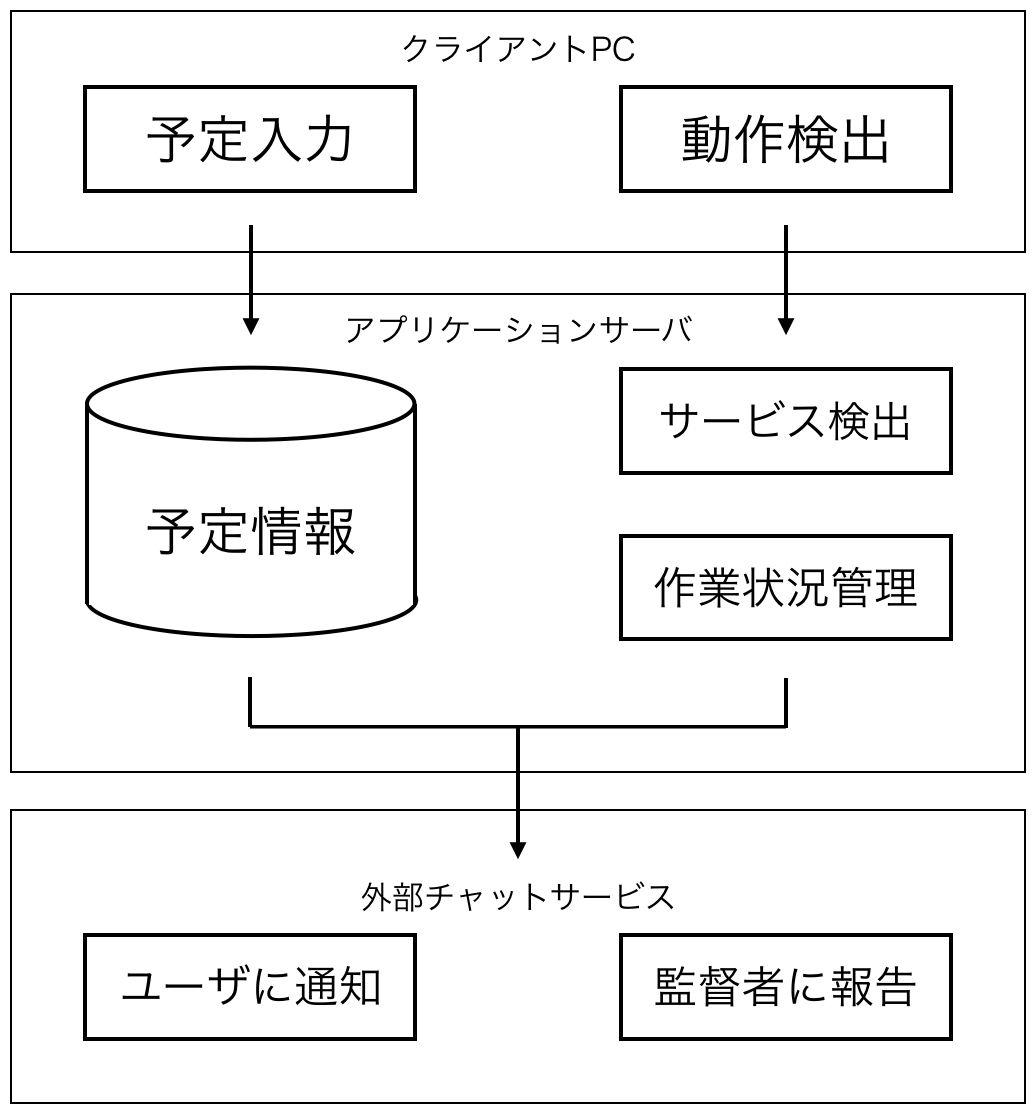
\includegraphics[width=12.0cm]{graphics/structure_chart.png}
  \caption{システム構成図}
  \label{fig:structure_chart}
  \end{center}
\end{figure}

\clearpage

\section{予定の管理機能}
ユーザは,システム利用開始時に,作業予定の設定を行う.
設定内容は,作業内容と作業の予定日時で構成される.
設定画面の一部を以下に示す

\begin{figure}[h]
  \begin{center}
  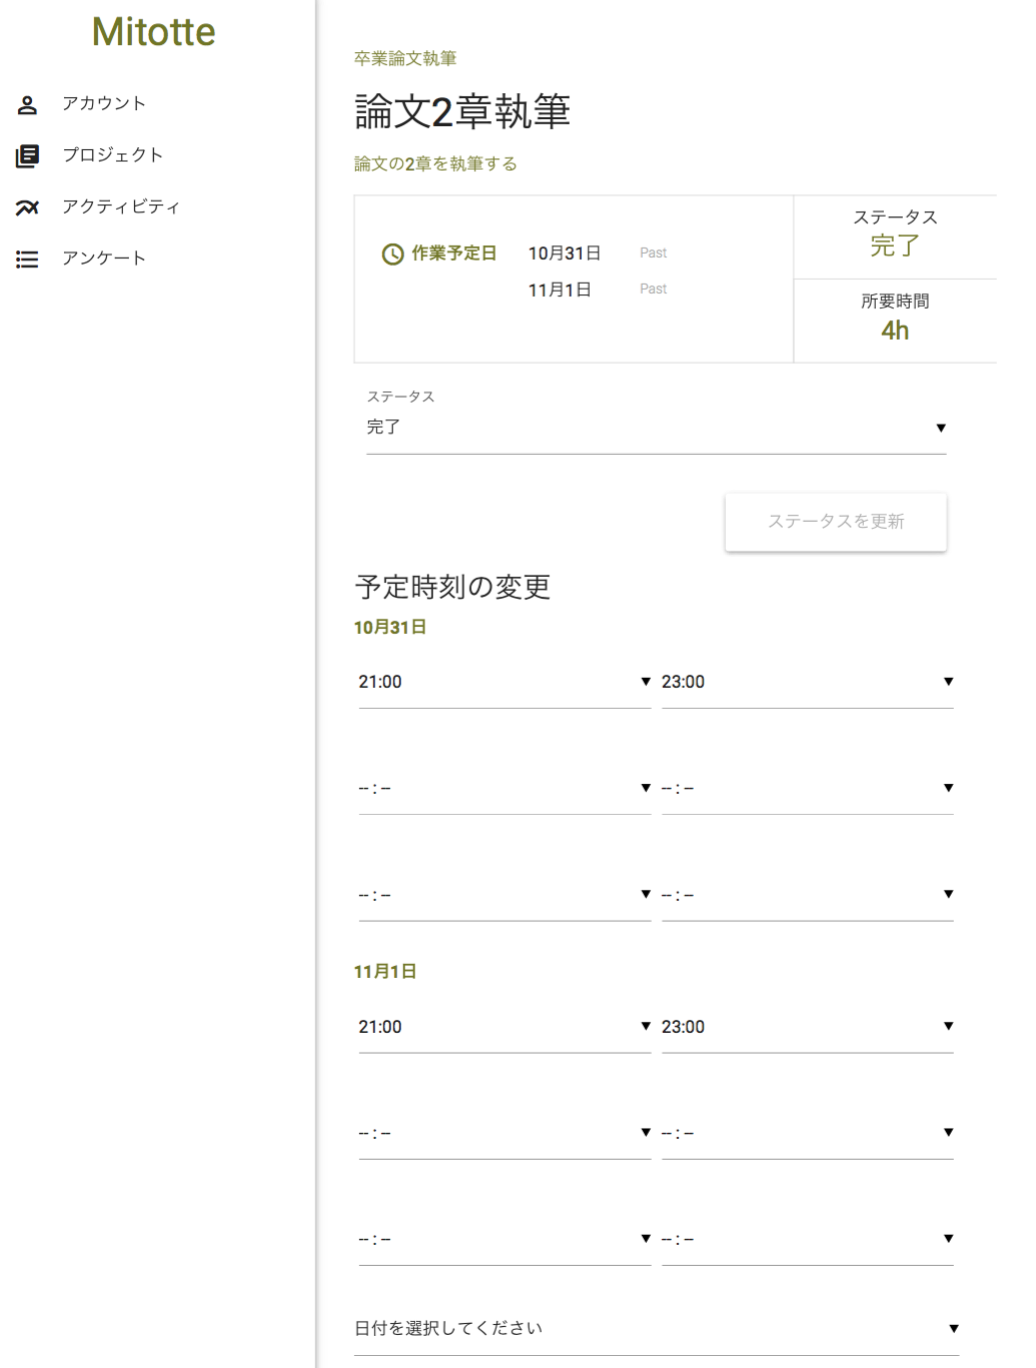
\includegraphics[width=12.0cm]{graphics/mitotte01.png}
  \caption{予定設定画面}
  \end{center}
\end{figure}

\clearpage

設定された作業予定やその作業のステータス(進行中,完了している,など)は
以下のように一覧で確認できる.

\begin{figure}[h]
  \begin{center}
  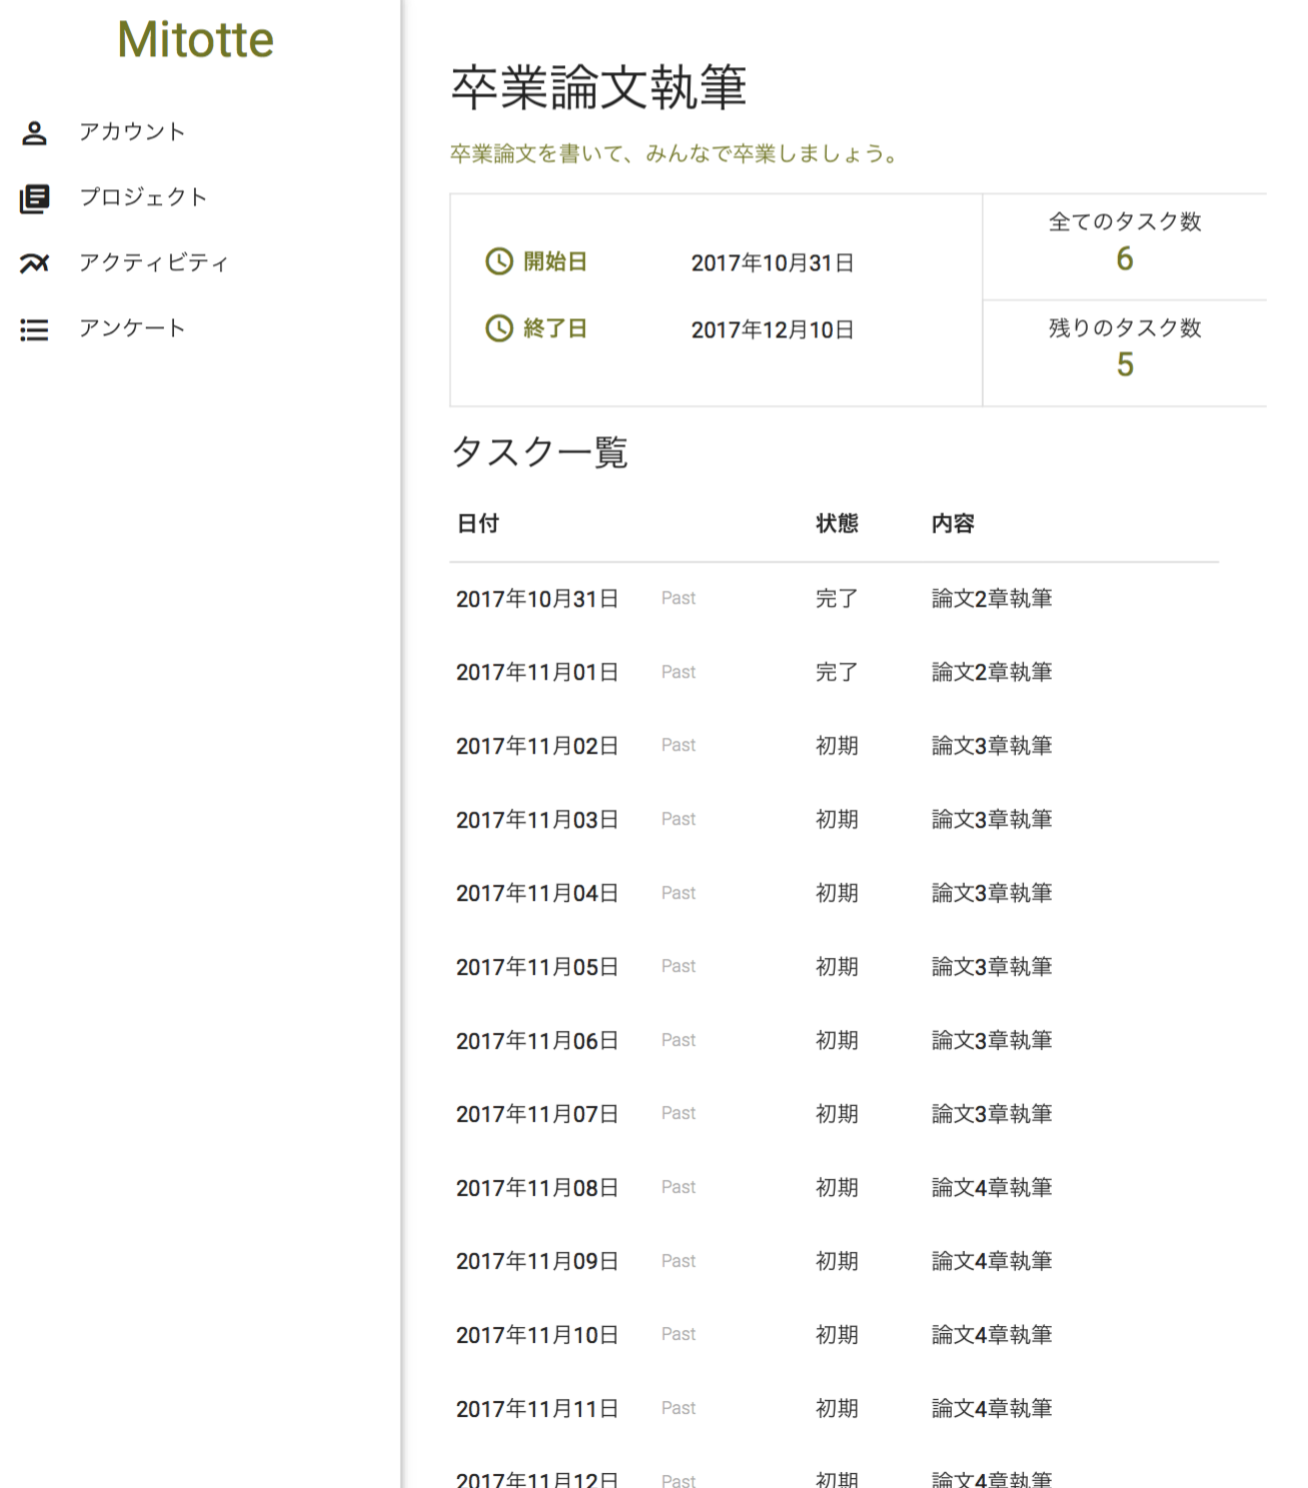
\includegraphics[width=12.0cm]{graphics/mitotte02.png}
  \caption{作業一覧画面}
  \end{center}
\end{figure}

設定された作業予定は,ユーザへの通知や,監督者へ状況を報告する際に利用される.
また,作業全体の進捗状況は,設定された予定が基準になっている.
ユーザはアプリケーション内でいつでも予定を変更可能であるが,予定を変更した履歴も監督者に通知される.

\section{アプリケーションによる監視}
本システムでは,アプリケーション内でPCを監視する際,ユーザの作業状況の記録及び,利用中のサービスの検出を行う.

\subsection{作業状況の記録}
アプリケーションの起動状況は,ユーザがバックグラウンドで本システムを起動させておくことで,自動的にサーバに記録される.
また,作業予定になっているもののうち,現在何の作業を行っているのかをユーザが能動的に記録することも可能である.
ただし,自動検知された起動状況は,ユーザ自身が書き換えることはできない.

\subsection{サービス検出}
本研究でのアプリケーションでは,ユーザのPC上で現在表示している画面から,サービスの検出を行う.
まず,アプリケーションが起動している間,ユーザがPC上の画面をキャプチャ画像として自動的に保存する.
その後サーバ上で,それらの画像を解析することにより,ユーザが利用しているサービスの検出を行う.
画像の解析は,Google社のサービスである, Google Cloud Vision API (以下,Vision API)を利用する.

ユーザの画面キャプチャ画像を Vision API に通すことにより,その画像内に含まれるモノ,テキスト情報,サービスのロゴ画像等を検出する.
それらの情報を元に,ユーザが作業に不要なサービスを利用していないかの判別を行う.

\clearpage

キャプチャ画像から,Vision APIを通して情報を取得した例を示す.

\begin{figure}[h]
  \begin{center}
  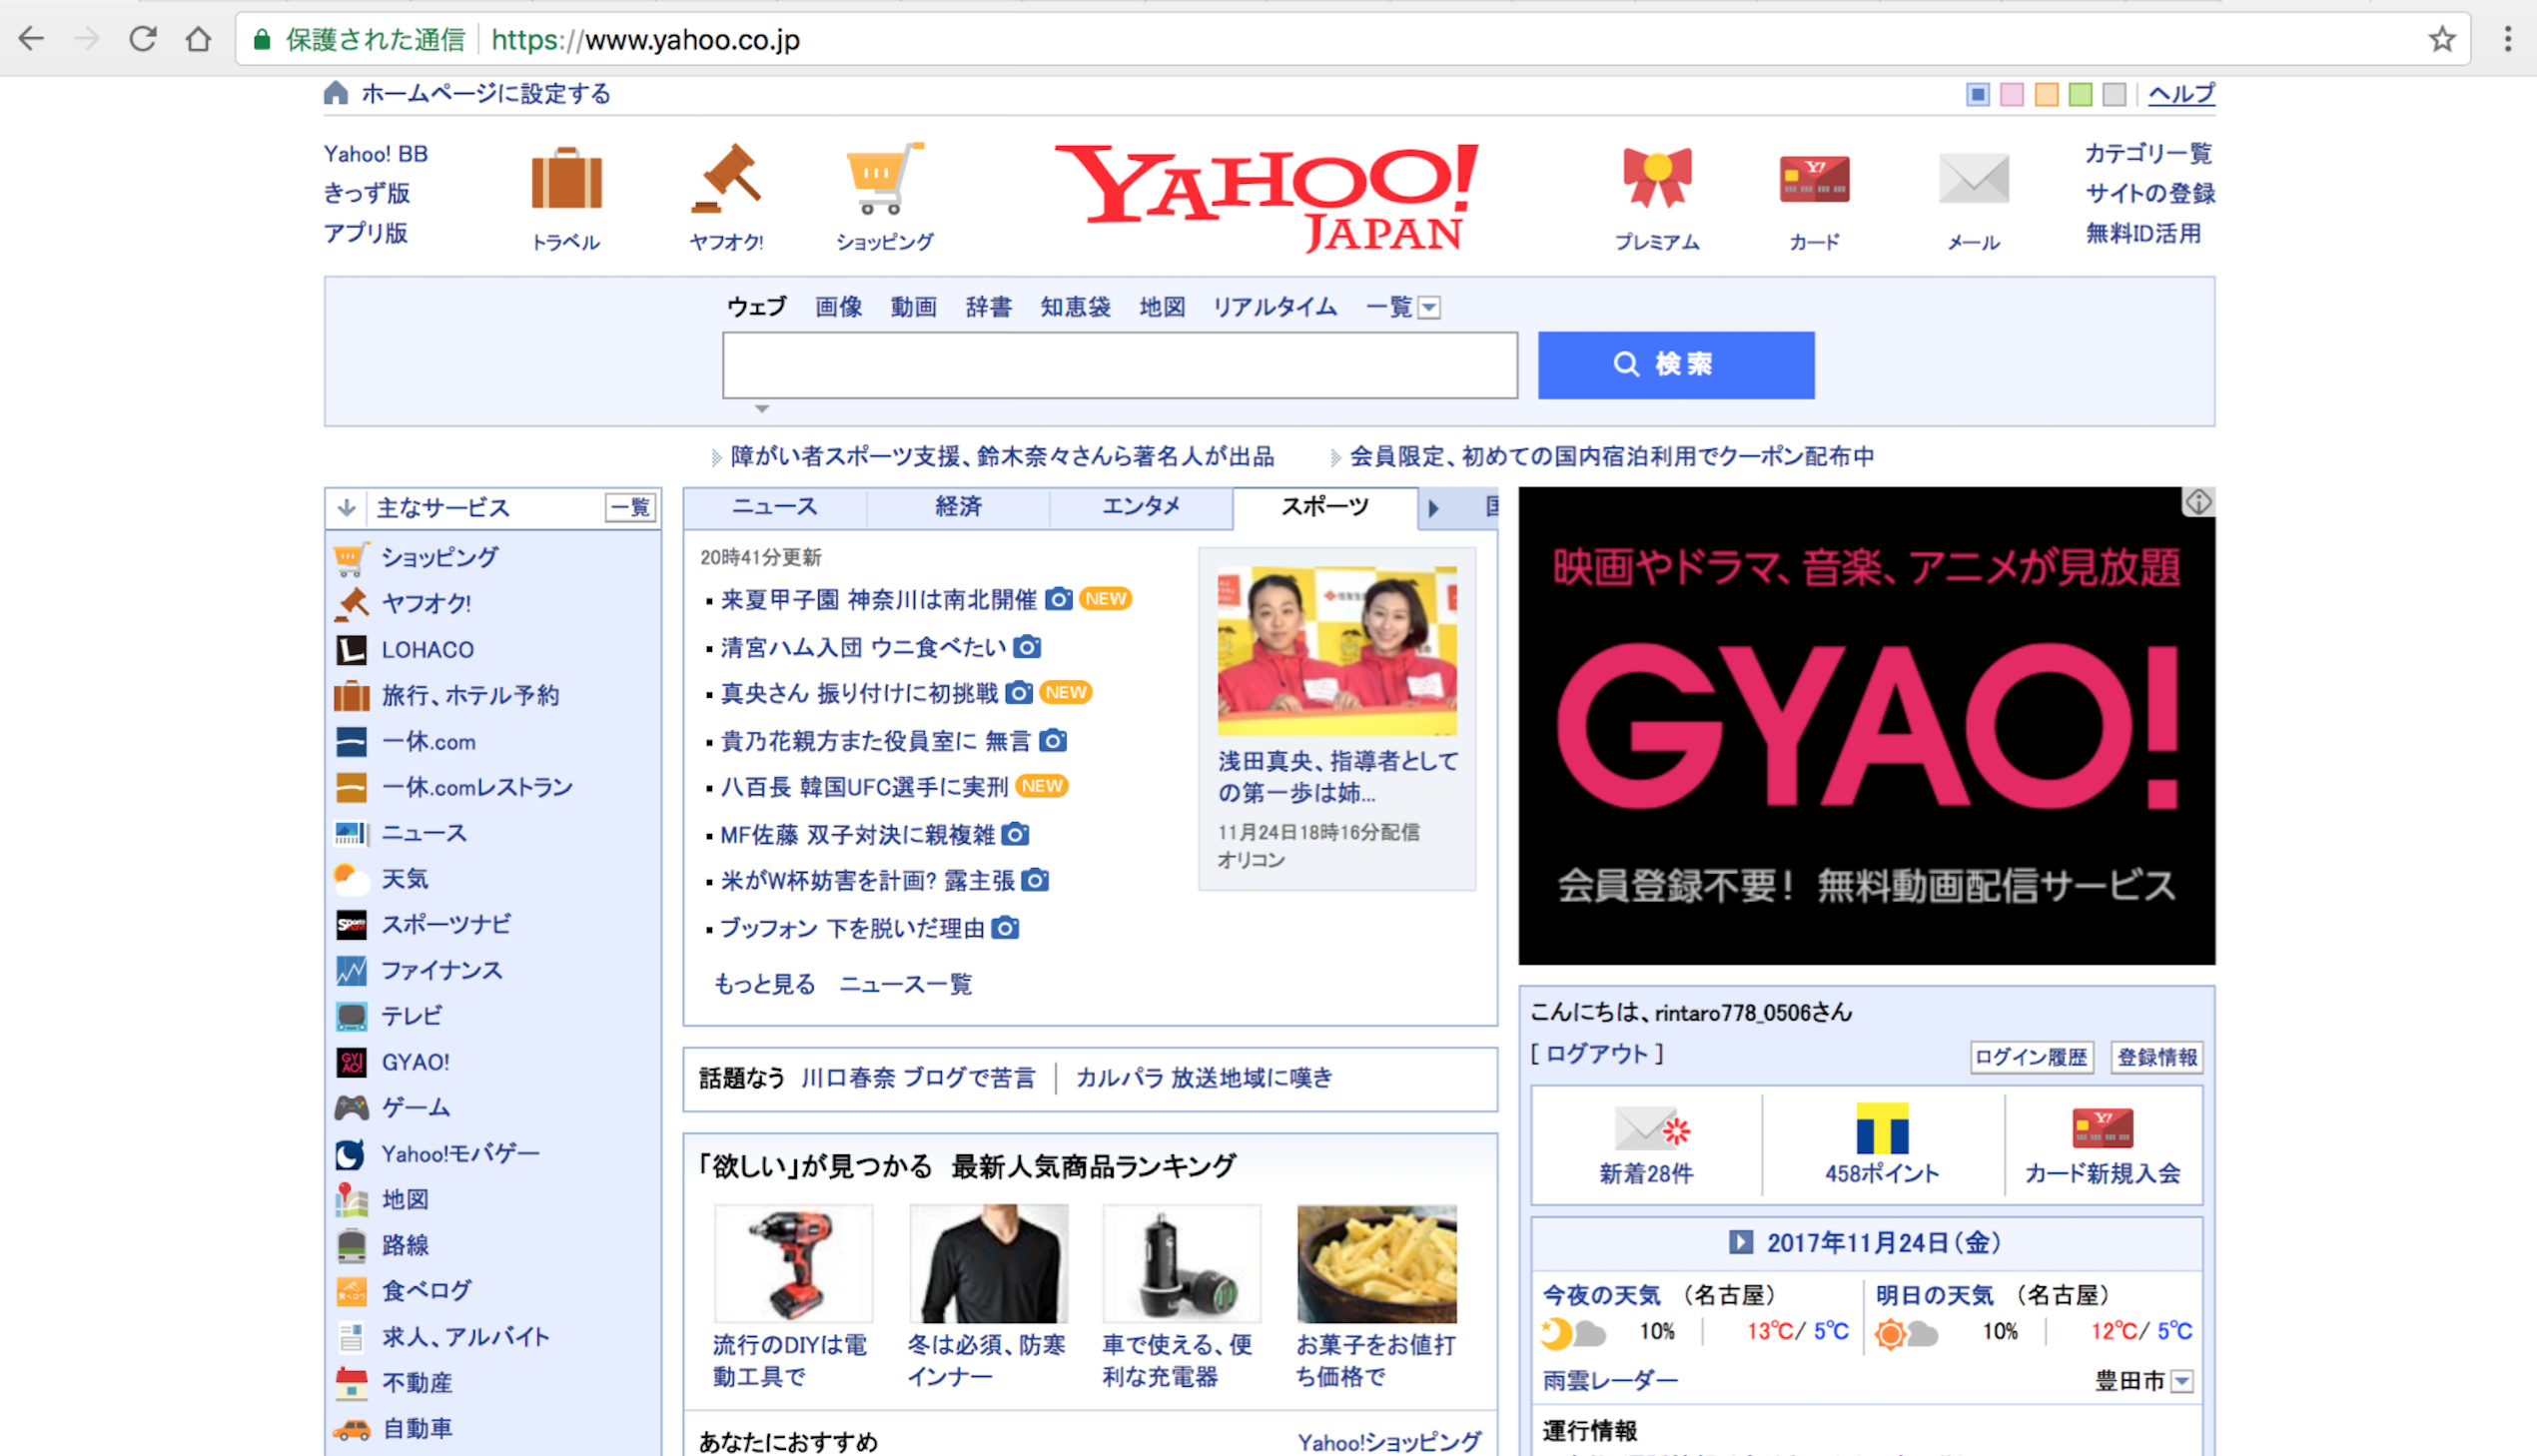
\includegraphics[width=14.0cm]{graphics/screenshot01.png}
  \caption{キャプチャ画像1}
  \label{fig:screenshot01}
  \end{center}
\end{figure}

キャプチャ画像1(図\ref{fig:screenshot01})では,以下のような情報が検出される.
ユーザがWebサイトを閲覧していることが分かる.

\begin{figure}[h]
  \begin{center}
  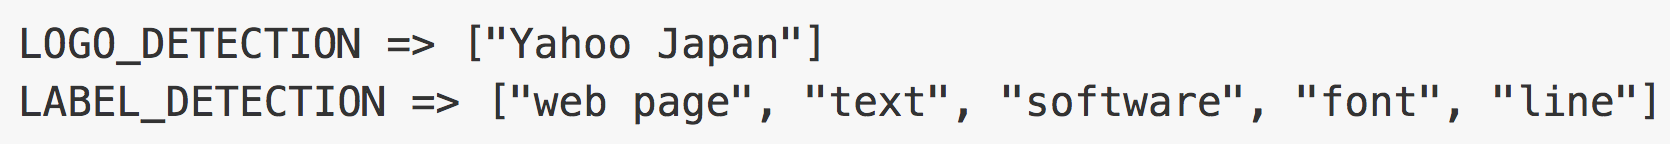
\includegraphics[width=14.0cm]{graphics/response01.png}
  \caption{検出された情報1}
  \label{fig:response01}
  \end{center}
\end{figure}

\clearpage

\begin{figure}[h]
  \begin{center}
  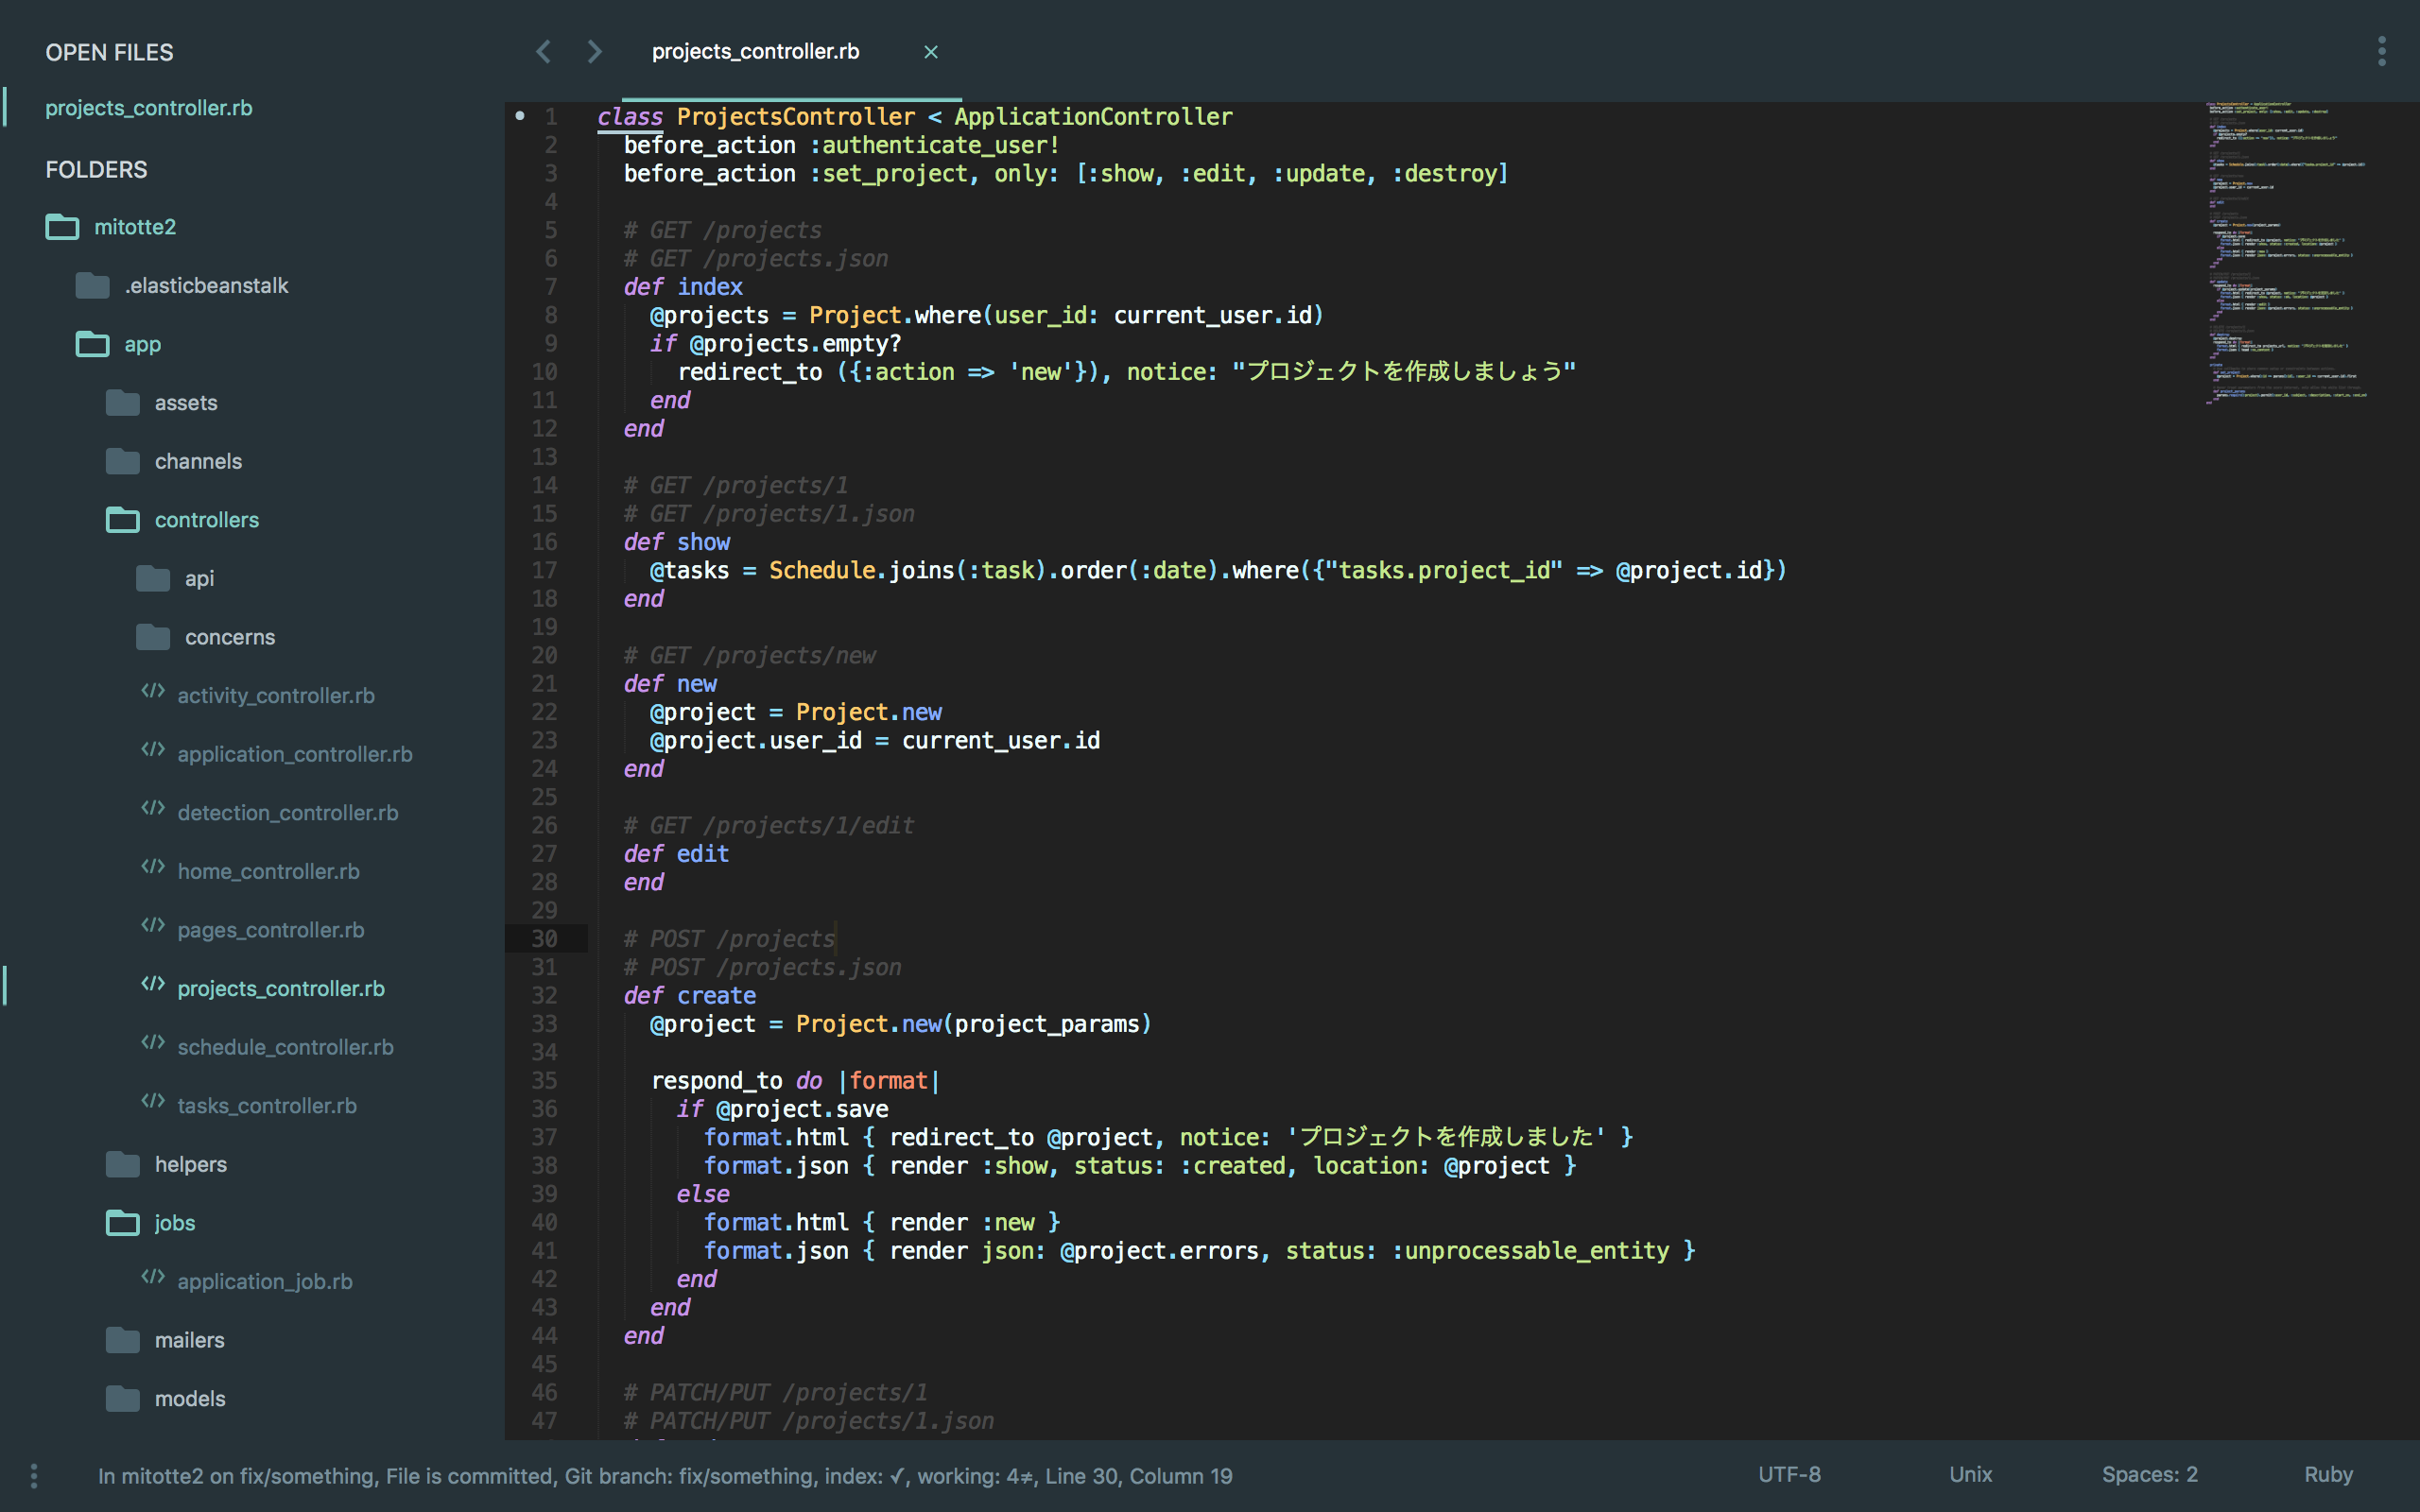
\includegraphics[width=14.0cm]{graphics/screenshot02.png}
  \caption{キャプチャ画像2}
  \label{fig:screenshot02}
  \end{center}
\end{figure}

キャプチャ画像2(図\ref{fig:screenshot02})では,以下のような情報が検出される.
ユーザがPC上のアプリケーションでプログラムのソースコードを表示していることを検出していることが分かる.

\begin{figure}[h]
  \begin{center}
  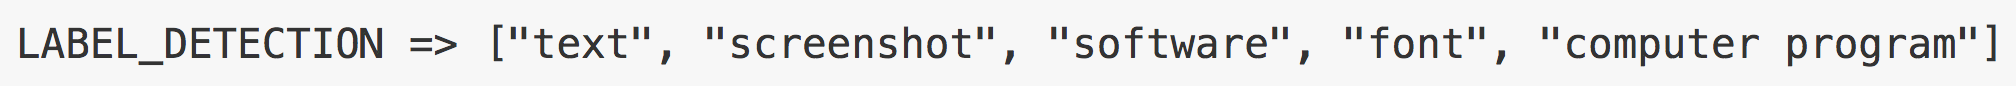
\includegraphics[width=14.0cm]{graphics/response02.png}
  \caption{検出された情報2}
  \label{fig:response02}
  \end{center}
\end{figure}

Vision APIから取得したこれらの情報を用いて,サービスの検出を行う.

\subsection{通知}
アプリケーションからユーザ及び監督者へ通知には,外部のチャットサービスを利用する.
まず,設定された作業予定時に,ユーザに対して通知が送信される.
ユーザは,チャットサービスから受け取る通知により,作業時間であることを認識できる.
通知後,アプリケーション上で動作が確認できなかった場合,30分毎に通知を繰り返す.
それによって,継続的にユーザに対して作業を開始することを促すことができる.

\begin{figure}[h]
  \begin{center}
  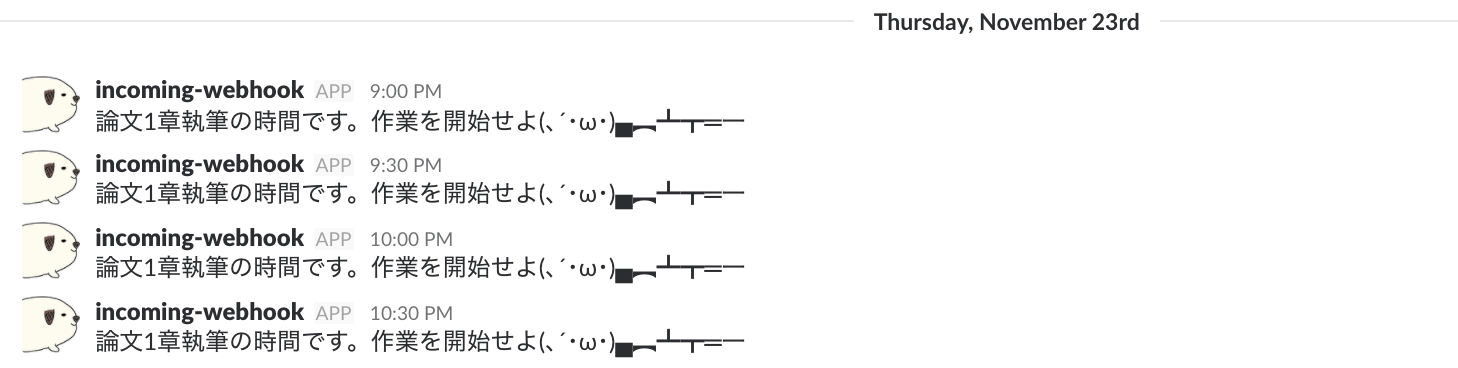
\includegraphics[width=14.0cm]{graphics/notification01.png}
  \caption{ユーザへの通知}
  \end{center}
\end{figure}

また,1日に1回決まった時刻に,前日の作業記録を監督者に通知する.
監督者は前日の作業記録を確認することにより,ユーザが作業を行った時間や,作業状況を把握できる.

\begin{figure}[h]
  \begin{center}
  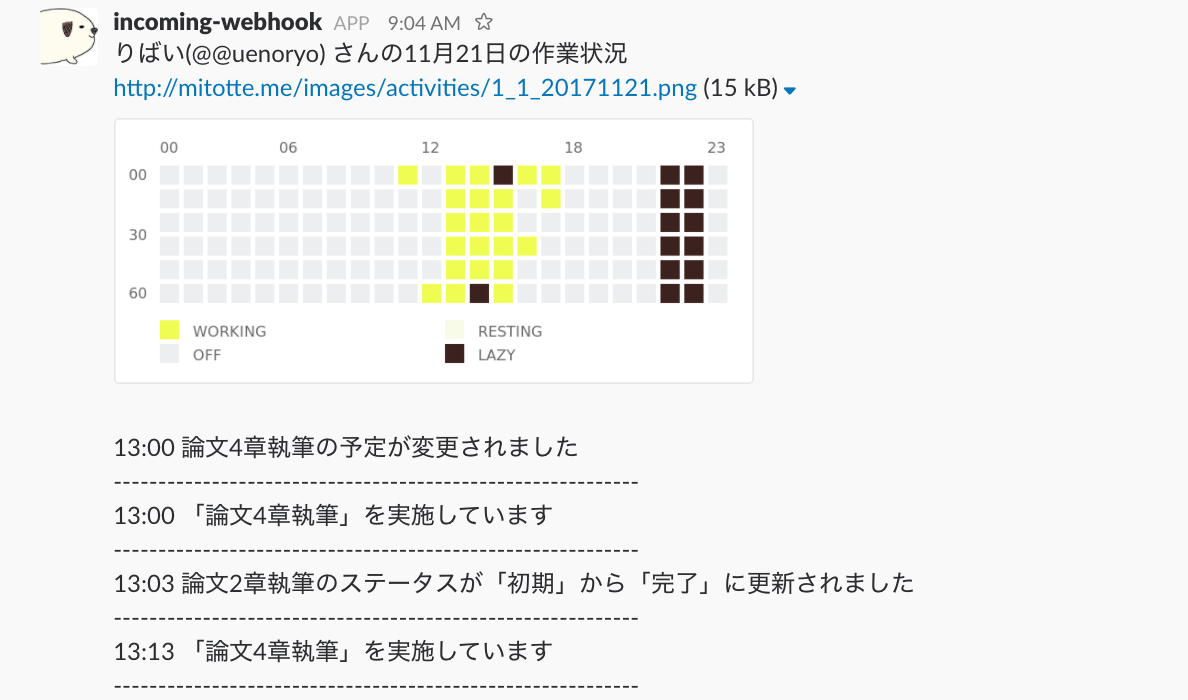
\includegraphics[width=14.0cm]{graphics/notification02.png}
  \caption{監督者への通知}
  \end{center}
\end{figure}

\clearpage

\section{作業記録の生成}
ユーザは,アプリケーション内で常に自分の作業状況を確認できる.
作業記録は,主に2種類の形式で生成される.

1つは図\ref{fig:activity_table}のように,作業時間をテーブル上に色分けしたものである.
テーブルからは,ユーザが作業を行っていた時間や,作業の予定時間内に作業ができていなかった時間が確認できる.

\begin{figure}[h]
  \begin{center}
  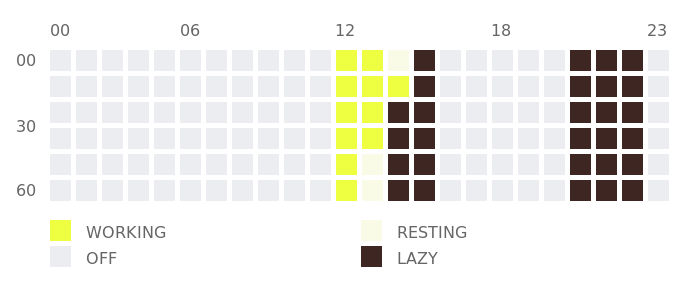
\includegraphics[width=12.0cm]{graphics/activity_table.png}
  \caption{作業時間のテーブル}
  \label{fig:activity_table}
  \end{center}
\end{figure}

\clearpage

2つ目は,ユーザのアプリケーション内の動作を記録した情報である.
図\ref{fig:activity_log}のように,動作の検出時間と,内容をリスト形式で表示する.
これらの作業記録はすべて監督者への通知でも利用される.

\begin{figure}[h]
  \begin{center}
  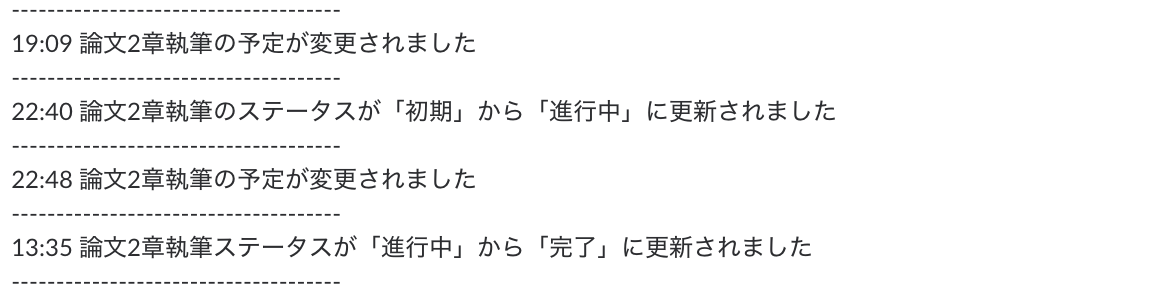
\includegraphics[width=14.0cm]{graphics/activity_log.png}
  \caption{作業時間のテーブル}
  \label{fig:activity_log}
  \end{center}
\end{figure}
